\documentclass{beamer}
\usetheme{Madrid}
\usecolortheme{albatross}

\usepackage[polish]{babel}
\usepackage[utf8]{inputenc}
\usepackage[T1]{fontenc}
\usepackage{graphicx}
\usepackage{booktabs}
\usepackage{longtable}
\usepackage{comment}

% --- Dane projektu ---
\title[RehabSense]{RehabSense - System wspomagania rehabilitacji}
\author[RT, KB, MM, KH, KR]{
    Remigiusz Tomecki \and Kacper Błaszczyk \and Maciej Miazek \\
    Klim Hudzenko \and Kacper Romek
}
\institute[PŁ]{Politechnika Łódzka}
\date{1 kwietnia 2026}

\begin{document}

% 1. Strona tytułowa
\begin{frame}
    \titlepage
\end{frame}

% 2. Cel Projektu
\begin{frame}{Cel Projektu}
    \begin{itemize}
        \item Stworzenie inteligentnego interfejsu człowiek–maszyna do analizy zachowań i ruchu użytkownika.
        \item Wsparcie procesu diagnostyki, terapii i rehabilitacji poprzez zwiększenie precyzji oceny ruchowej.
        \item Ułatwienie monitorowania postępów i ograniczenie błędów wynikających z manualnych obserwacji.
        \item Zaliczenie przedmiotu.
    \end{itemize}
\end{frame}

% 3. Analiza Problemu
\begin{frame}{Analiza Problemu}
    \begin{itemize}
        \item \textbf{Brak nadzoru w domu:} Pacjenci często wykonują ćwiczenia nieprawidłowo bez nadzoru fizjoterapeuty, co może prowadzić do braku postępów lub pogłębienia urazów.
        \item \textbf{Ograniczone śledzenie postępów:} Trudność w obiektywnym i systematycznym pomiarze zakresu ruchu pacjenta poza gabinetem.
        \item \textbf{Niewystarczająca komunikacja:} Brak dedykowanych, zintegrowanych platform do płynnej wymiany informacji między pacjentem a specjalistą na odległość.
        \item \textbf{Spadek motywacji:} Monotonia ćwiczeń domowych oraz brak natychmiastowej informacji zwrotnej prowadzą do zniechęcenia i porzucania rehabilitacji.
    \end{itemize}
\end{frame}

% 4. Pomysł na Aplikację
\begin{frame}{Pomysł na Aplikację}
    \begin{itemize}
        \item Aplikacja webowa umożliwiająca naśladowanie ćwiczeń rehabilitacyjnych wyświetlanych na ekranie.
        \item Cel aplikacji to nadzorowanie poprawności wykonywanych ćwiczeń rehabilitacyjnych.
        \item Aplikacja rozpoznaje postawę ciała użytkownika z użyciem \textbf{google-ai-edge/mediapipe}, analizuje ją, sprawdzając czy ćwiczenia są wykonywane poprawnie.
        \item Aplikacja monitoruje postępy w rehabilitacji sprawdzając np. czy zakres ruchu użytkownika się poprawia również używając mediapipe.
        \item RehabSense umożliwia założenie konta Pacjenta lub Fizjoterapeuty (Fizjoterapeuta dodaje Pacjentowi ćwiczenia do wykonania oraz ma dostęp do sprawdzania jego postępów).
    \end{itemize}
\end{frame}

% 5. Analiza istniejących rozwiązań - Moje Fizjo Plus
\begin{frame}{Analiza istniejących rozwiązań: Moje Fizjo Plus}
    \begin{itemize}
        \item \textbf{Zalety:}
        \begin{itemize}
            \item Zestawy ćwiczeń przygotowane przez ekspertów wraz z filmikami instruktażowymi.
            \item Testy dopasowywujące poziom ćwiczeń, wprowadza testy palpacyjne wraz z filmami instruktażowymi. W celu zminimalizowania pogłębienia kontuzji lub wad postawy przez wykonywanie ćwiczeń.
            \item Intuicyjny i przyjemny interfejs użytkownika.
        \end{itemize}
        \item \textbf{Wady:}
        \begin{itemize}
            \item Brak wsparcia dla kamery i rozpoznawania pozycji ciała, w celu kontroli poprawności wykonywania ćwiczeń.
            \item Ograniczenie się do osób borykających się z dolegliwościami bólowymi kręgosłupa, barku i biodra.
            \item Brak wsparcia dla kontaktu między fizjoterapeutami a pacjentami.
        \end{itemize}
    \end{itemize}
\end{frame}

% 5. Analiza istniejących rozwiązań - Physiapp
\begin{frame}{Analiza istniejących rozwiązań: Physiapp}
    \begin{itemize}
        \item \textbf{Zalety:}
        \begin{itemize}
            \item Łączenie fizjoterapeutów z pacjentami.
            \item Śledzenie postępów.
            \item System passy (zachęta do regularnego wykonywania ćwiczeń).
            \item Intuicyjny i przyjemny interfejs użytkownika.
        \end{itemize}
        \item \textbf{Wady:}
        \begin{itemize}
            \item Brak możliwości korzystania z aplikacji bez kodu.
            \item Brak wsparcia dla kamery i rozpoznawania pozycji ciała, w celu kontroli poprawności wykonywania ćwiczeń.
        \end{itemize}
    \end{itemize}
\end{frame}

% 5. Analiza istniejących rozwiązań - Kaia Health
\begin{frame}{Analiza istniejących rozwiązań: Kaia Health}
    \begin{itemize}
        \item \textbf{Zalety:}
        \begin{itemize}
            \item Przygotowane zestawy ćwiczeń terapeutycznych.
            \item Analizowanie pozycji ciała i zakresu ruchów, dając feedback w czasie rzeczywistym wykonywania ćwiczenia.
            \item Łączenie pacjentów z fizjoterapeutami poprzez chat tekstowy i wideo.
            \item Możliwość śledzenia progresu.
        \end{itemize}
        \item \textbf{Wady:}
        \begin{itemize}
            \item Aplikacja jest płatna.
            \item Do korzystania z aplikacji wymagane jest podanie nazwy firmy lub ubezpieczyciela (ale też innych danych jak np. maila pracowniczego, stanowiska).
        \end{itemize}
    \end{itemize}
\end{frame}

% 5. Analiza istniejących rozwiązań - Freeletics
\begin{frame}{Analiza istniejących rozwiązań: Freeletics}
    \begin{itemize}
        \item \textbf{Zalety:}
        \begin{itemize}
            \item Dopasowywanie planów treningowych z użyciem AI.
            \item Szeroka gama zastosowań aplikacji: plany treningowe tworzone są na podstawie krótkiej ankiety i dopasowywane do użytkownika. Utworzony plan treningowy może być nastawiony na budowanie masy mięśniowej, odchudzanie lub powrót do formy.
            \item Wsparcie wykonywania ćwiczeń za pomocą kamery i rozpoznawania zakresów ruchu z użyciem AI.
            \item Dostosowanie planów treningowych do sprzętu użytkownika.
        \end{itemize}
        \item \textbf{Wady:}
        \begin{itemize}
            \item Model subskrypcyjny aplikacji, brak dostępu do aplikacji bez wybrania płatnego planu subskrypcji.
            \item Aplikacja nie wspomaga bezpośrednio procesu rehabilitacji, a jest raczej nastawiona na ćwiczenia dla osób zdrowych.
        \end{itemize}
    \end{itemize}
\end{frame}

% 6. Wymagania Funkcjonalne
\begin{frame}{Wymagania Funkcjonalne (1/2)}
    \footnotesize
    \begin{itemize}
        \item \textbf{WF1.} Użytkownik może się zarejestrować i zalogować
        \item \textbf{WF2.} System zapewnia użytkownikowi jedną z 2 ról: pacjent lub fizjoterapeuta
        \item \textbf{WF3.} Pacjent ma dostęp do panelu statystyk swojej rehabilitacji
        \item \textbf{WF4.} Komunikacja między pacjentem a fizjoterapeutą (czat tekstowy)
        \item \textbf{WF5.} Pacjent ma dostęp do planu rehabilitacji
        \item \textbf{WF6.} Pacjent może wykonać sesję ćwiczeń
        \item \textbf{WF7.} System nagradza pacjenta za regularność i jakość wykonywania ćwiczeń (passa, punkty)
    \end{itemize}
\end{frame}

\begin{frame}{Wymagania Funkcjonalne (2/2)}
    \footnotesize
    \begin{itemize}
        \item \textbf{WF8.} Fizjoterapeuta może przeglądać listę swoich pacjentów
        \item \textbf{WF9.} Fizjoterapeuta może tworzyć i przypisywać spersonalizowane plany ćwiczeń dla pacjentów
        \item \textbf{WF10.} Fizjoterapeuta ma dostęp do panelu statystyk swoich pacjentów (problem, historia rehabilitacji, postęp)
        \item \textbf{WF11.} System porównuje w czasie rzeczywistym ruch użytkownika ze wzorcem danego ćwiczenia
        \item \textbf{WF12.} System aktualizuje postęp rehabilitacji po zakończonej sesji
        \item \textbf{WF13.} Administrator może dodawać zweryfikowanych* fizjoterapeutów do bazy
        \item \textbf{WF14.} System zarządza danymi fizjoterapeuty, do których należą co najmniej: imię i nazwisko, specjalizacja oraz posiadane certyfikaty
    \end{itemize}
    \vspace{0.3cm}
    \scriptsize * weryfikacja fizjoterapeutów odbywa się poza aplikacją
\end{frame}

% 6. Wymagania Niefunkcjonalne
\begin{frame}{Wymagania Niefunkcjonalne}
    \begin{itemize}
        \item \textbf{WNF1.} System powinien działać stabilnie – błędy nie powodują zatrzymania działania aplikacji.
        \item \textbf{WNF2.} Dokładność analizy na poziomie niemniejszym niż 75\%.
        \item \textbf{WNF3.} System zapewnia bezpieczeństwo dla danych użytkowników poprzez szyfrowanie.
        \item \textbf{WNF4.} Intuicyjny interfejs - dostęp do najważniejszych komponentów aplikacji w maksymalnie pięciu kliknięciach.
        \item \textbf{WNF5.} Integracja z innymi aplikacjami poprzez API.
        \item \textbf{WNF6.} Do prawidłowego działania systemu potrzebna jest kamerka internetowa.
    \end{itemize}
\end{frame}

% 7. Diagram przypadków użycia
\begin{frame}{Diagram przypadków użycia}
    \begin{center}
        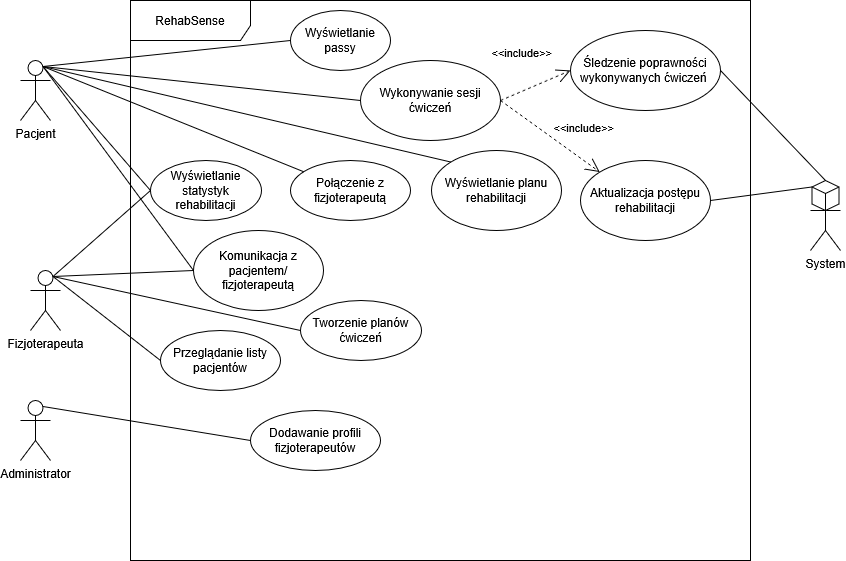
\includegraphics[width=0.9\textwidth,height=0.8\textheight,keepaspectratio]{files/przypadki.png}
    \end{center}
\end{frame}

% 8. Scenariusze Przypadków Użycia
\begin{frame}{Scenariusz Przypadku Użycia}
    \tiny % zmiana na najmniejszą możliwą czcionkę w LaTeXu
    \begin{longtable}{|p{0.22\textwidth}|p{0.73\textwidth}|}
    	\hline
    	\textbf{Nazwa} & \textbf{Parowanie pacjenta i fizjoterapeuty} \\ \hline
    	\textbf{Numer} & 1 \\ \hline
    	\textbf{Twórca} & Zespół Projektowy \\ \hline
    	\textbf{Poziom ważności} & Wysoki \\ \hline
    	\textbf{Typ przypadku użycia} & Ogólny \\ \hline
    	\textbf{Aktorzy} & \textbf{Pacjent}, \textbf{Fizjoterapeuta}, \textbf{System} \\ \hline
    	\textbf{Krótki opis} & Proces automatycznego doboru fizjoterapeuty przez system na podstawie potrzeb pacjenta oraz zatwierdzenie połączenia. \\ \hline
    	\textbf{Warunki wstępne} & 
    	$\bullet$ Pacjent i Fizjoterapeuta są zarejestrowani.\newline
    	$\bullet$ Pacjent jest zalogowany do systemu.
    	\\ \hline
    	\textbf{Warunki końcowe} & Profile pacjenta i fizjoterapeuty zostają pomyślnie i trwale połączone w aplikacji. \\ \hline
    	\textbf{Główny przepływ zdarzeń} & 
    	1. Pacjent rozpoczyna proces szukania fizjoterapeuty poprzez wybranie odpowiedniej opcji i określenie swojego problemu.\newline
    	2. System dobiera fizjoterapeutę, którego specjalizacja odpowiada potrzebom pacjenta oraz jest dostępny.\newline
    	3. Wybrany fizjoterapeuta zatwierdza prośbę na podstawie informacji o pacjencie.\newline
    	4. Pacjent ostatecznie zatwierdza wybranego specjalistę co skutkuje połączeniem ich profili.
    	\\ \hline
    	\textbf{Alternatywne przepływy zdarzeń} & 
    	\textbf{3a.} Jeśli fizjoterapeuta odrzuci prośbę lub nie odpowie w określonym czasie, system automatycznie wybierze innego specjalistę, a proces wraca do kroku 2. \\ \hline
    	\textbf{Specjalne wymagania} & Optymalny i szybki algorytm filtrujący dla znalezienia idealnego specjalisty. \\ \hline
    	\textbf{Notatki i kwestie} & Brak. \\ \hline
    	\caption{Scenariusz przypadku użycia: Parowanie pacjenta i fizjoterapeuty}
    \end{longtable}
\end{frame}

\begin{frame}[allowframebreaks]{Diagram Sekwencji}
	\begin{center}
		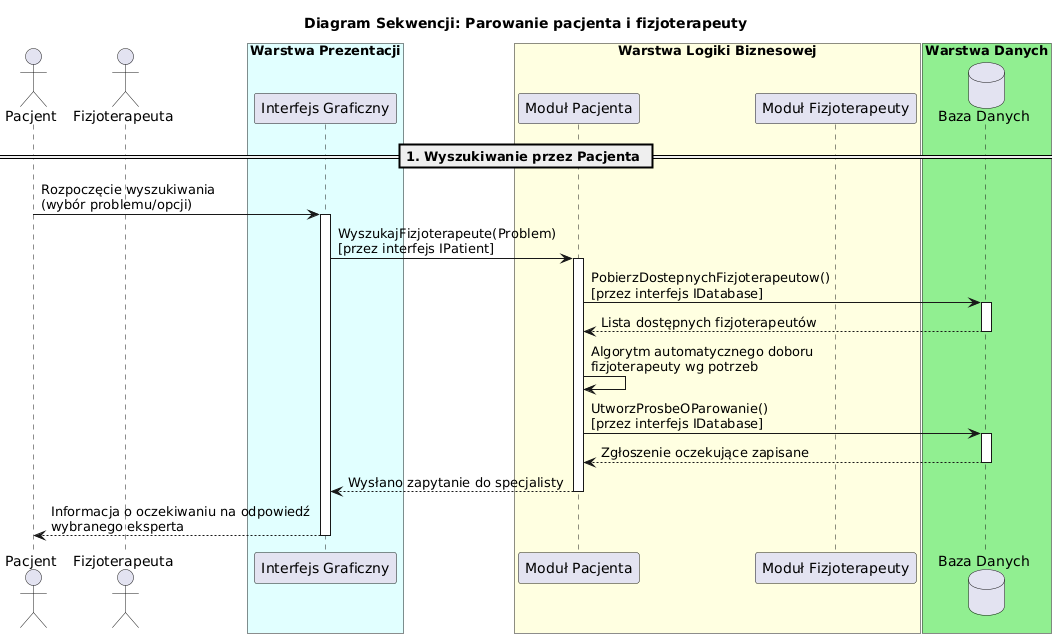
\includegraphics[width=0.9\textwidth,height=0.8\textheight,keepaspectratio]{files/sekwencji_1.png}
	\end{center}

	\begin{center}
		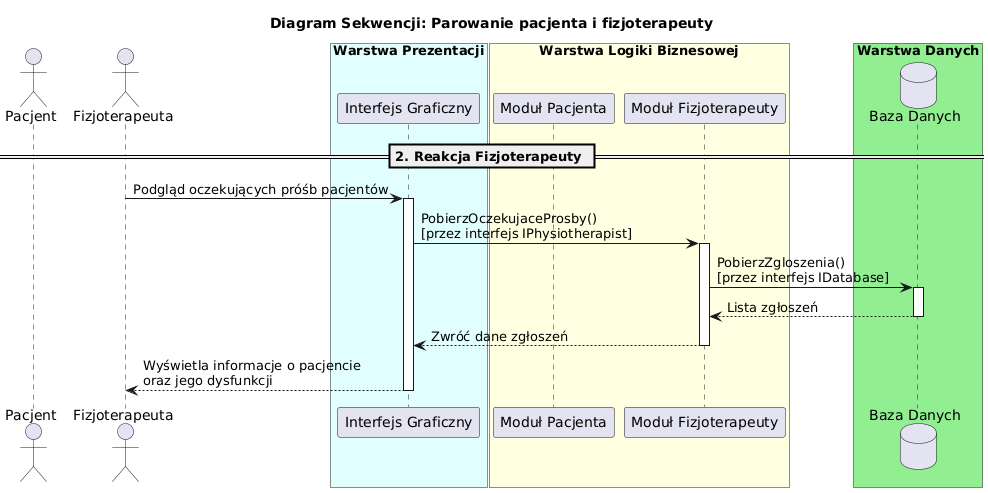
\includegraphics[width=0.9\textwidth,height=0.8\textheight,keepaspectratio]{files/sekwencji_2.png}
	\end{center}

	\begin{center}
		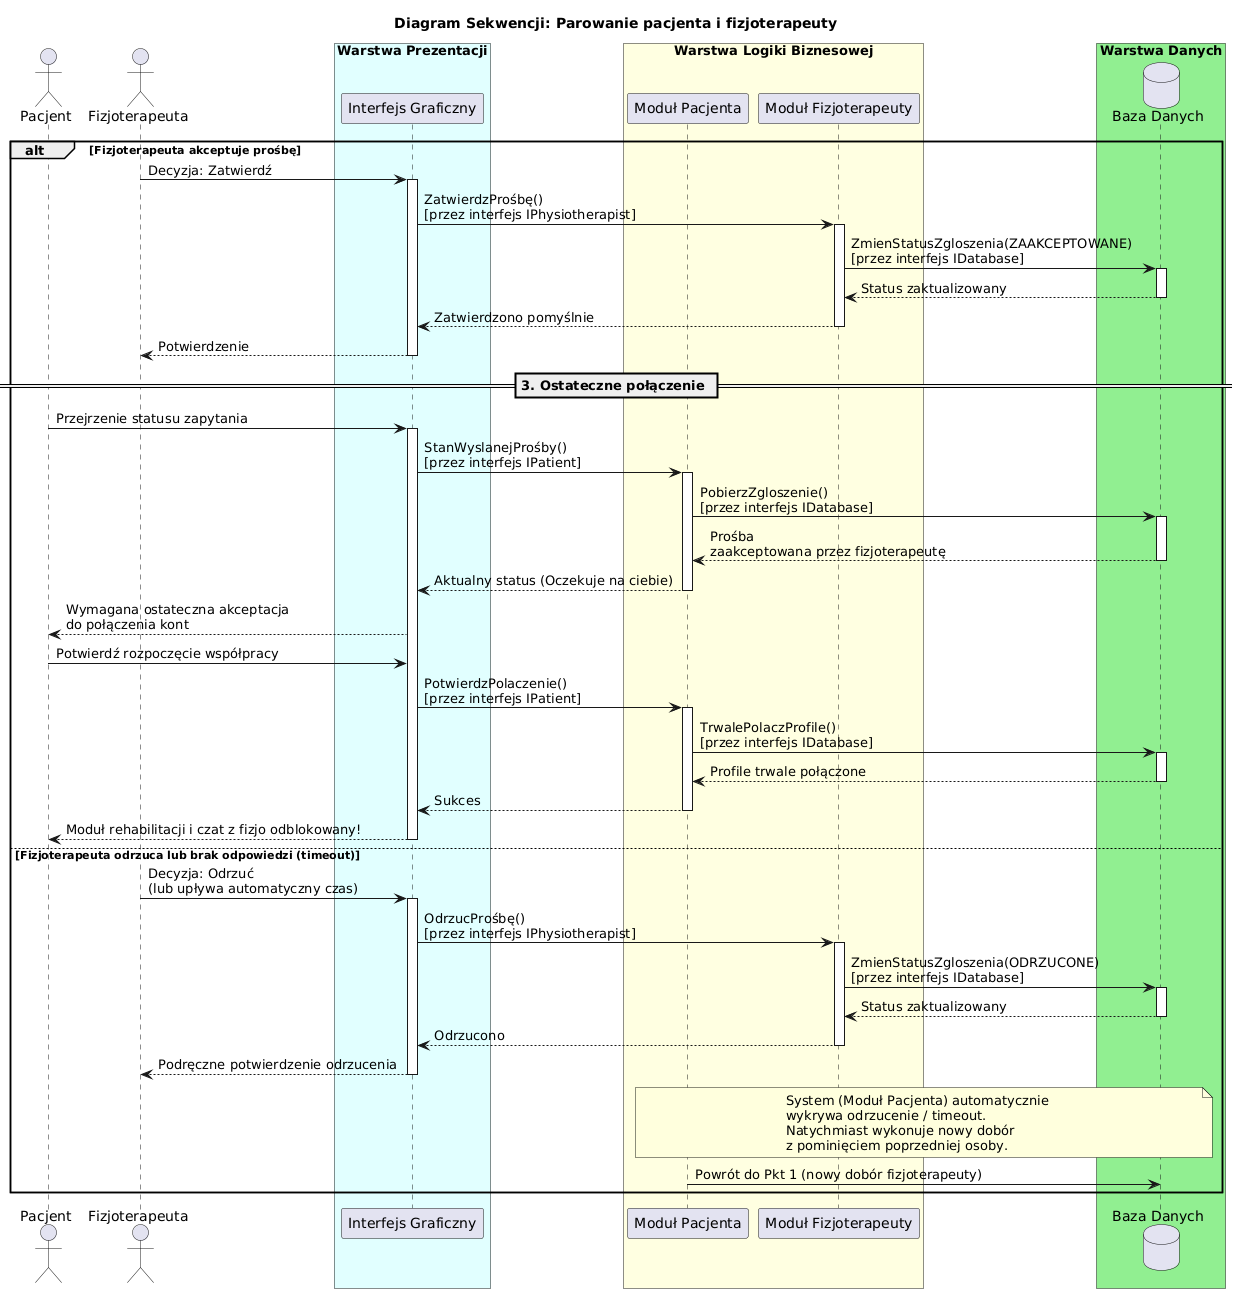
\includegraphics[width=0.9\textwidth,height=0.8\textheight,keepaspectratio]{files/sekwencji_3.png}
	\end{center}
\end{frame}

\begin{comment}
\begin{frame}[allowframebreaks]{Scenariusze Przypadków Użycia - c.d.}
    \tiny % zmiana na najmniejszą możliwą czcionkę w LaTeXu
    \begin{longtable}{|p{0.22\textwidth}|p{0.73\textwidth}|}
    	\hline
    	\textbf{Nazwa} & \textbf{Przeglądanie listy pacjentów} \\ \hline
    	\textbf{Numer} & 2 \\ \hline
    	\textbf{Twórca} & Zespół Projektowy \\ \hline
    	\textbf{Poziom ważności} & Średni \\ \hline
    	\textbf{Typ przypadku użycia} & Ogólny \\ \hline
    	\textbf{Aktorzy} & \textbf{Fizjoterapeuta}, \textbf{System} \\ \hline
    	\textbf{Krótki opis} & Umożliwienie fizjoterapeucie przeglądu przypisanych mu pacjentów oraz selekcji konta do wglądu w statystyki. \\ \hline
    	\textbf{Warunki wstępne} & 
    	$\bullet$ Fizjoterapeuta jest zalogowany do systemu.\newline
    	$\bullet$ Fizjoterapeuta ma przypisanego co najmniej jednego pacjenta.
    	\\ \hline
    	\textbf{Warunki końcowe} & Wyświetlona zostaje lista dostępnych do analizy pacjentów, a specjalista może przejść do wybranego profilu. \\ \hline
    	\textbf{Główny przepływ zdarzeń} & 
    	1. Fizjoterapeuta wybiera zakładkę z listą przypisanych pacjentów.\newline
    	2. System weryfikuje powiązania w bazie i pobiera odpowiednie konta pacjentów.\newline
    	3. System wyświetla wizualnie listę pacjentów wraz z ich podstawowymi statystykami (czas aktywności itp.).\newline
    	4. Fizjoterapeuta wybiera konkretnego pacjenta, aby przejść do szczegółowych danych jego rehabilitacji.
    	\\ \hline
    	\textbf{Alternatywne przepływy zdarzeń} & 
    	\textbf{2a.} Brak przypisanych pacjentów: System informuje o pustej liście i wyświetla ewentualne instrukcje dla pracownika. \\ \hline
    	\textbf{Specjalne wymagania} & Szybki, asynchroniczny czas odpowiedzi przy wyświetleniu dużej ilości kont. \\ \hline
    	\textbf{Notatki i kwestie} & Brak. \\ \hline
    	\caption{Scenariusz przypadku użycia: Przeglądanie listy pacjentów}
    \end{longtable}
\end{frame}
\end{comment}

% 9. Architektura Rozwiązania
\begin{frame}{Architektura Rozwiązania - Warstwy}
    System został podzielony na trzy główne warstwy:
    \begin{itemize}
        \item \textbf{Prezentacji} – interfejs użytkownika.
        \item \textbf{Logiki biznesowej} – procesy i moduły funkcjonalne.
        \item \textbf{Danych} – centralne repozytorium informacji.
    \end{itemize}
    \vspace{0.4cm}
    \textbf{Warstwa Prezentacji:}
    Komponent Interfejs Graficzny stanowi punkt wejścia dla grup: Pacjent, Fizjoterapeuta, Administrator. Zaprojektowany intuicyjnie – dostęp do kluczowych funkcji w max. 5 kliknięciach.
\end{frame}

\begin{frame}{Architektura - Logika Biznesowa}
    Warstwa składająca się z czterech głównych modułów:
    \begin{itemize}
        \item \textbf{Moduł Pacjenta:} Rejestracja, materiały instruktażowe, zarządzanie planem rehabilitacji. Realizuje funkcję "systemu passy" nagradzającą za regularność.
        \item \textbf{Moduł Fizjoterapeuty:} Zarządzanie listą pacjentów, tworzenie spersonalizowanych planów ćwiczeń, wgląd w statystyki (problem, historia, postęp).
        \item \textbf{Moduł AI:} Wykorzystuje model \textit{google-ai-edge/mediapipe} do analizy obrazu w czasie rzeczywistym. Porównuje ruch ze wzorcem (dokładność min. 75\%). Wyniki aktualizują historię postępów.
        \item \textbf{Moduł Administracji:} Zarządzanie bazą zweryfikowanych fizjoterapeutów. Pozwala na ręczne dodawanie specjalistów po zewnętrznej weryfikacji.
    \end{itemize}
\end{frame}

\begin{frame}{Architektura - Warstwa Danych}
    Pełni rolę centralnego repozytorium informacji. Przechowuje:
    \begin{itemize}
        \item Dane o profilach użytkowników i połączenia (Pacjent-Fizjo).
        \item Materiały wideo oraz plany treningowe.
        \item Historię wyników z modułu AI.
    \end{itemize}
\end{frame}

% 10. Diagram Komponentów
\begin{frame}{Diagram Komponentów}
    \begin{center}
		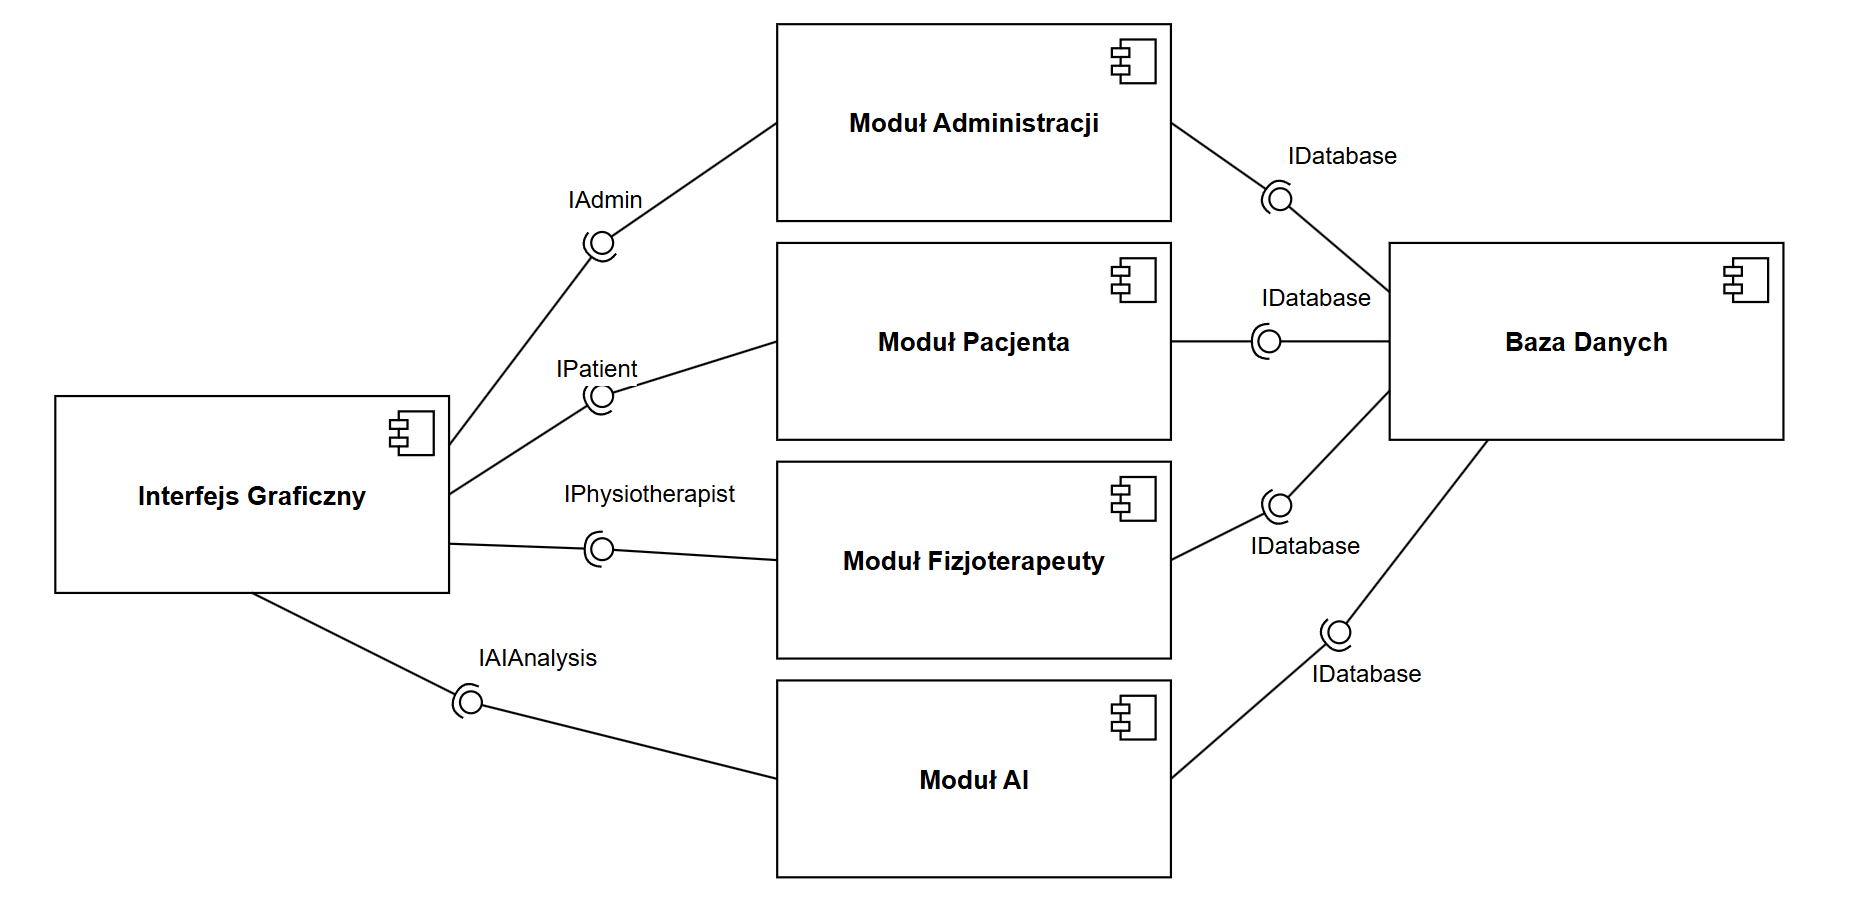
\includegraphics[width=0.9\textwidth,height=0.8\textheight,keepaspectratio]{files/kompo.png}
	\end{center}
\end{frame}

\begin{frame}{Diagram Bazy Danych}
    \begin{center}
		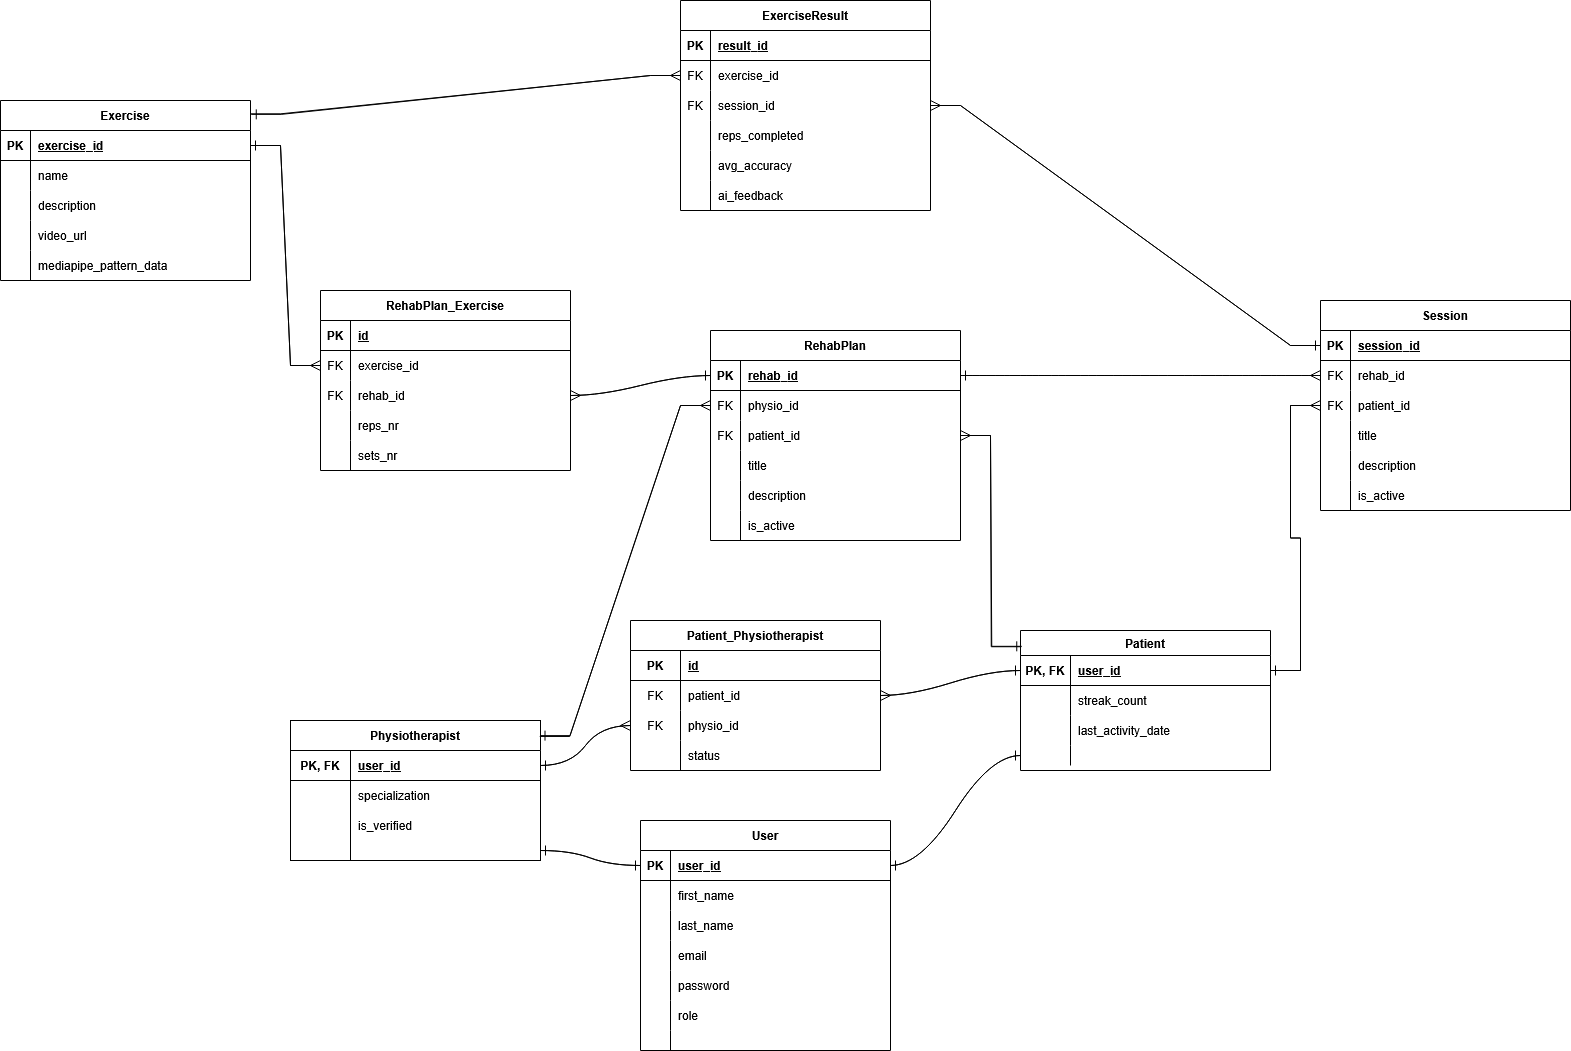
\includegraphics[width=0.9\textwidth,height=0.8\textheight,keepaspectratio]{files/bazka.png}
	\end{center}
\end{frame}

\begin{frame}{Stack Technologiczny}
	\textbf{Backend}
	\begin{itemize}
		\item Python
	\end{itemize}
	\textbf{Frontend}
	\begin{itemize}
		\item Next.js
		\item Tailwind CSS
	\end{itemize}
\end{frame}

% 11. Harmonogram Prac
\begin{frame}{Harmonogram Prac}
   	\begin{table}
   		\small
   		\centering
   		\begin{tabular}{|l|c|p{5.5cm}|}
   			\hline
   			\textbf{Faza} & \textbf{Tydzień} & \textbf{Kluczowe Zadania} \\ \hline
   			1. Analiza & 1 -- 4 & Zbieranie wymagań, specyfikacja, architektura. \\ \hline
   			2. Projektowanie & 5 -- 8 & UX/UI, baza danych, logika biznesowa. \\ \hline
   			3. Implementacja & 9 -- 16 & Frontend, backend, integracja. \\ \hline
   			4. Testowanie & 17 -- 20 & Testy funkcjonalne i niefunkcjonalne, naprawa błędów. \\ \hline
   			5. Wdrożenie & 21 -- 24 & Szkolenia, produkcja, wsparcie techniczne. \\ \hline
   		\end{tabular}
   	\end{table}
\end{frame}

% 12. Podział na Role
\begin{frame}{Podział na Role}
    \begin{center}
        \Large
        $\left.
        \begin{tabular}{@{}l@{}}
             Remigiusz Tomecki \\
             Kacper Błaszczyk \\
             Maciej Miazek \\
             Klim Hudzenko \\
             Kacper Romek
        \end{tabular}
        \right\}$ \textbf{Full-Stack}
    \end{center}
\end{frame}

% 13. Zakończenie
\begin{frame}
    \begin{center}
        \Huge Dziękujemy za uwagę :)
    \end{center}
\end{frame}

\end{document}